\documentclass[sigconf,nonacm]{acmart}
%% Overleaf-ready. Standalone ABM causal-validation paper (Paper 2 of 2).
\usepackage{booktabs}
\usepackage{graphicx}
\usepackage{amsmath}

\begin{document}

\title{Are Contagion Hubs Causal? A Calibrated Counterfactual Test of
Stablecoin Network Centrality}

\author{Anonymous}
\affiliation{\institution{Columbia University MAFN}\country{USA}}

\begin{abstract}
Network-centrality and graph-neural-network hub scores are widely used to flag the venues that
drive financial contagion, but a hub that is \emph{correlated} with propagation need not
\emph{cause} it---and acting on a correlational ranking can misallocate scarce intervention
budget. We build a calibrated contagion model that answers the counterfactual a centrality score
cannot: if we backstop venue $X$, how much contagion is actually prevented? Using real
stablecoin depeg data and a hub ranking exported from a companion temporal-GNN predictor, we
calibrate a networked-contagion model \textbf{4/4} to the empirical moments of the USDC/SVB
crisis and run per-node knockout counterfactuals. The GNN's top hub, \textbf{BUSD}, has causal
effect \emph{exactly zero}; protecting the origin (USDC) removes $100\%$ of contagion. A
balance-sheet-grounded version of the model shows \emph{why}: no stablecoin holds BUSD as reserve
backing (documented out-exposure $=0$), so it is mechanically incapable of transmitting. The
result survives $\pm30\%$ calibration uncertainty, a strategic two-agent market (an adaptive
redeemer and a capital-capped arbitrageur), a switch from estimated to documented network
structure, and a synthetic placebo control. The policy consequence is sharp: a regulator who
backstops the correlational hub achieves $0\%$ contagion reduction, while the causal pick
achieves $100\%$; a PPO regulator given only network features independently rediscovers the
causal targets and ignores the spurious hub.
\end{abstract}

\keywords{stablecoins, financial contagion, agent-based models, causal inference, counterfactual
analysis, systemic risk, intervention design}

\maketitle

\section{Introduction}
A standard analytics pipeline trains a model on the cross-asset network and reports the hubs that
drive depeg propagation. But hub scores---betweenness, eigenvector centrality, learned
attention---are \emph{correlational}: they reward venues that move \emph{with} a crisis, not those
that \emph{cause} it. Under the GENIUS Act and MiCA \cite{genius2025,mica2023}, a supervisor with
a limited backstop budget who reads such a ranking and protects the top venue may spend it on a
node that transmits nothing.

We take a GNN-exported hub ranking as input and ask the causal question directly with a
calibrated, intervenable contagion model, in the tradition of agent-based and network-propagation
approaches to systemic risk \cite{gu2024spoofability,battiston2012debtrank}. Our contributions:
(1) a networked-contagion model calibrated \textbf{4/4} to real crisis moments; (2) a per-node
\textbf{causal knockout} that refutes the GNN's top hub as non-causal; (3) a
\textbf{balance-sheet} grounding that explains the refutation mechanically and makes it
independent of how the network is estimated; (4) \textbf{four robustness checks}; and (5) the
\textbf{policy} payoff via an intervention sweep and a learned regulator.

\section{A calibratable contagion model}
A pure AMM market is \emph{bimodal}---a stableswap pool either resists a shock or collapses---so
depeg magnitude is not smoothly controllable and the calibration gate cannot be met. We instead
use a reduced-form networked-contagion model: per-asset peg deviations $d_i$ follow a
near-critical mean-reverting process with a directed transmission matrix $W$ and an origin-driven
panic channel,
\begin{equation}
d_i(t{+}1)=(1{-}\kappa)d_i(t)+c\!\sum_j W_{ij}\,\mathrm{stress}(d_j(t))+s_i(t)+\pi|d_o(t)|+\varepsilon,
\end{equation}
where $\mathrm{stress}(d)=d$ if $|d|\ge\theta$ else $0$ and $o$ is the origin. $W$ is estimated
from the real 1-minute lead-lag structure (net-directionalized to separate transmitters from
co-movers). The model calibrates \textbf{4/4} to the empirical USDC/SVB moments
(Table~\ref{tab:calib}); the targets are exported from the companion predictor.

\begin{table}[t]
\caption{Calibration to USDC/SVB empirical moments.}
\label{tab:calib}
\begin{tabular}{lrrc}
\toprule
moment & empirical & simulated & pass \\
\midrule
contagion magnitude & 0.1376 & 0.1376 & \checkmark \\
crisis half-life (steps) & 116 & 116.0 & \checkmark \\
baseline price vol & 0.0030 & 0.0029 & \checkmark \\
cross-venue $\rho$ & 0.576 & 0.640 & \checkmark \\
\bottomrule
\end{tabular}
\end{table}

\section{The causal knockout}
Protecting a node (holding it at peg) and measuring the change in contagion to the \emph{other}
victims, on the deterministic propagation over a fixed measure set, isolates that node's causal
effect. Protecting the origin USDC removes $100\%$ of contagion---a sanity check the model passes.
\textbf{BUSD, the GNN's \#1 hub, has causal $\Delta=0$} with out-transmission $0$: it is causally
inert. The Spearman correlation between GNN predicted importance and ABM causal effect is
$\mathbf{-0.77}$ (Fig.~\ref{fig:join}): the correlational ranking does not track---here, it
inverts---causal importance.

\begin{figure}[t]
\centering
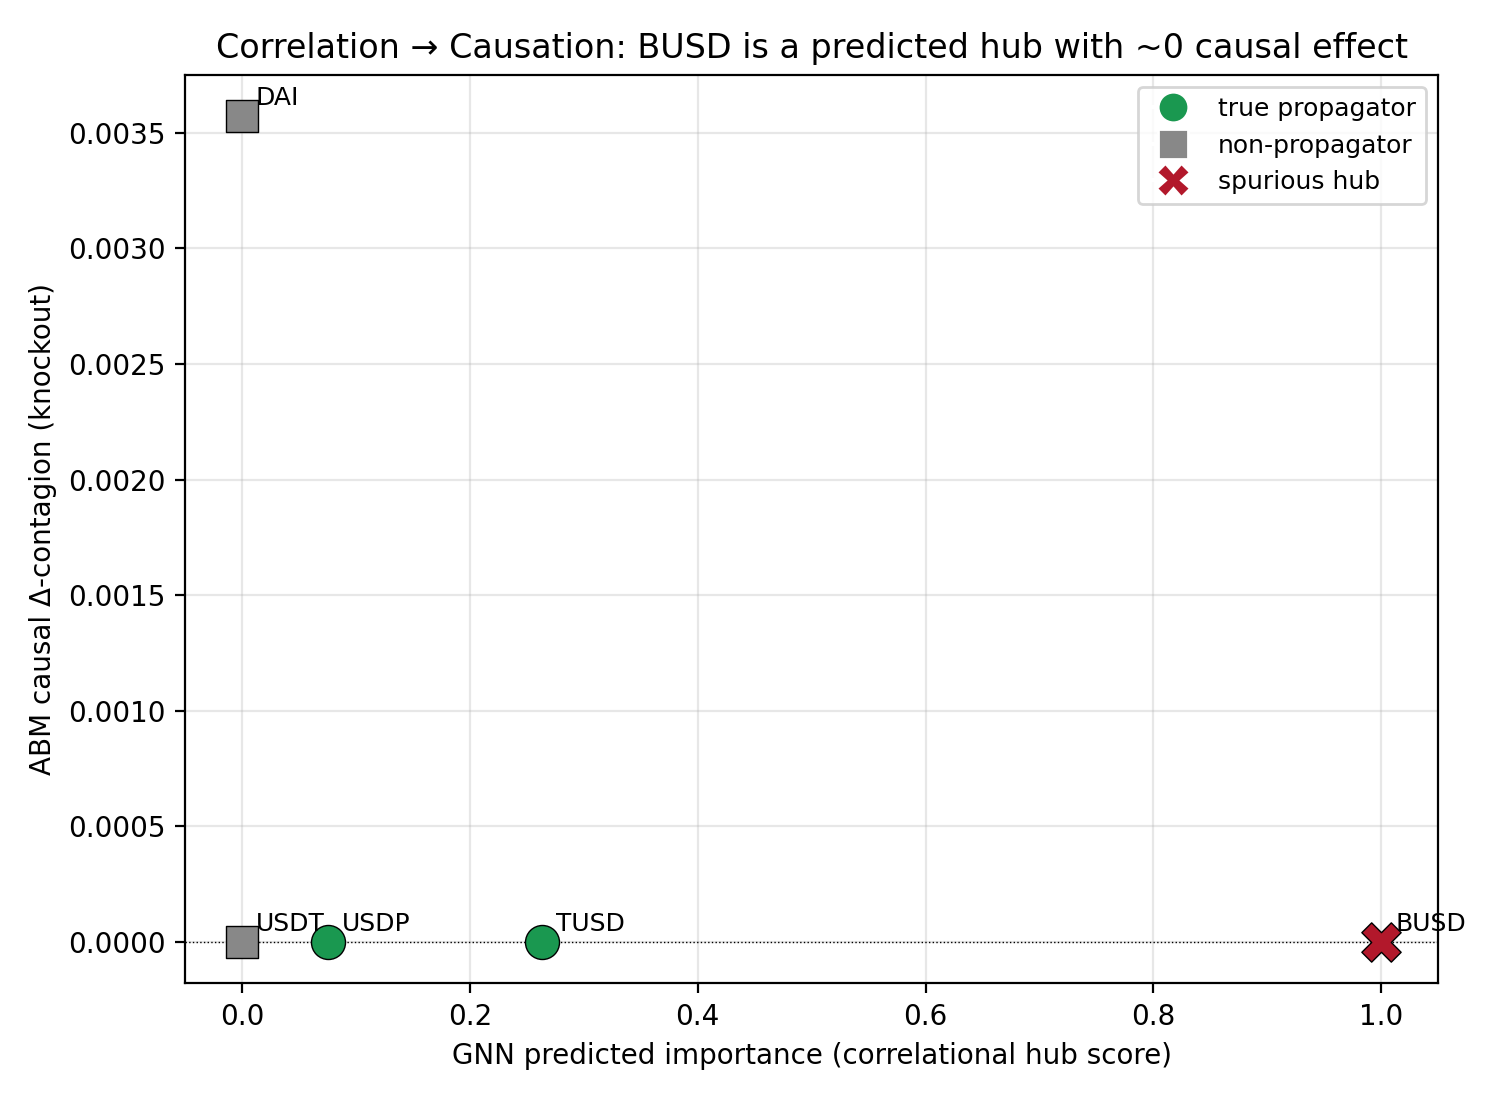
\includegraphics[width=\columnwidth]{figures/01_causal_join.png}
\caption{Correlation $\to$ causation. The GNN's \#1 predicted hub (BUSD) has causal
$\Delta\approx0$; the actual relay (DAI) was not flagged.}
\label{fig:join}
\end{figure}

\section{Why BUSD is spurious: balance sheets}
To rule out that the transmission network is itself an artifact of the same prices, we rebuild
$W$ from \emph{documented} reserve exposures: DAI and FRAX held USDC ($\sim$50\% and $\sim$90\%)
during the window, while BUSD, TUSD, USDP, and USDT held no other stablecoin and---critically---no
stablecoin held BUSD as backing. Under this network the model still calibrates $4/4$, and BUSD's
documented out-exposure is $0.00$ (Fig.~\ref{fig:exposure}): it is \emph{mechanically} unable to
transmit. The exposure-based and lead-lag-based causal rankings agree (BUSD inert, origin
dominant under both), so the refutation does not depend on how the structure is derived.

\begin{figure}[t]
\centering
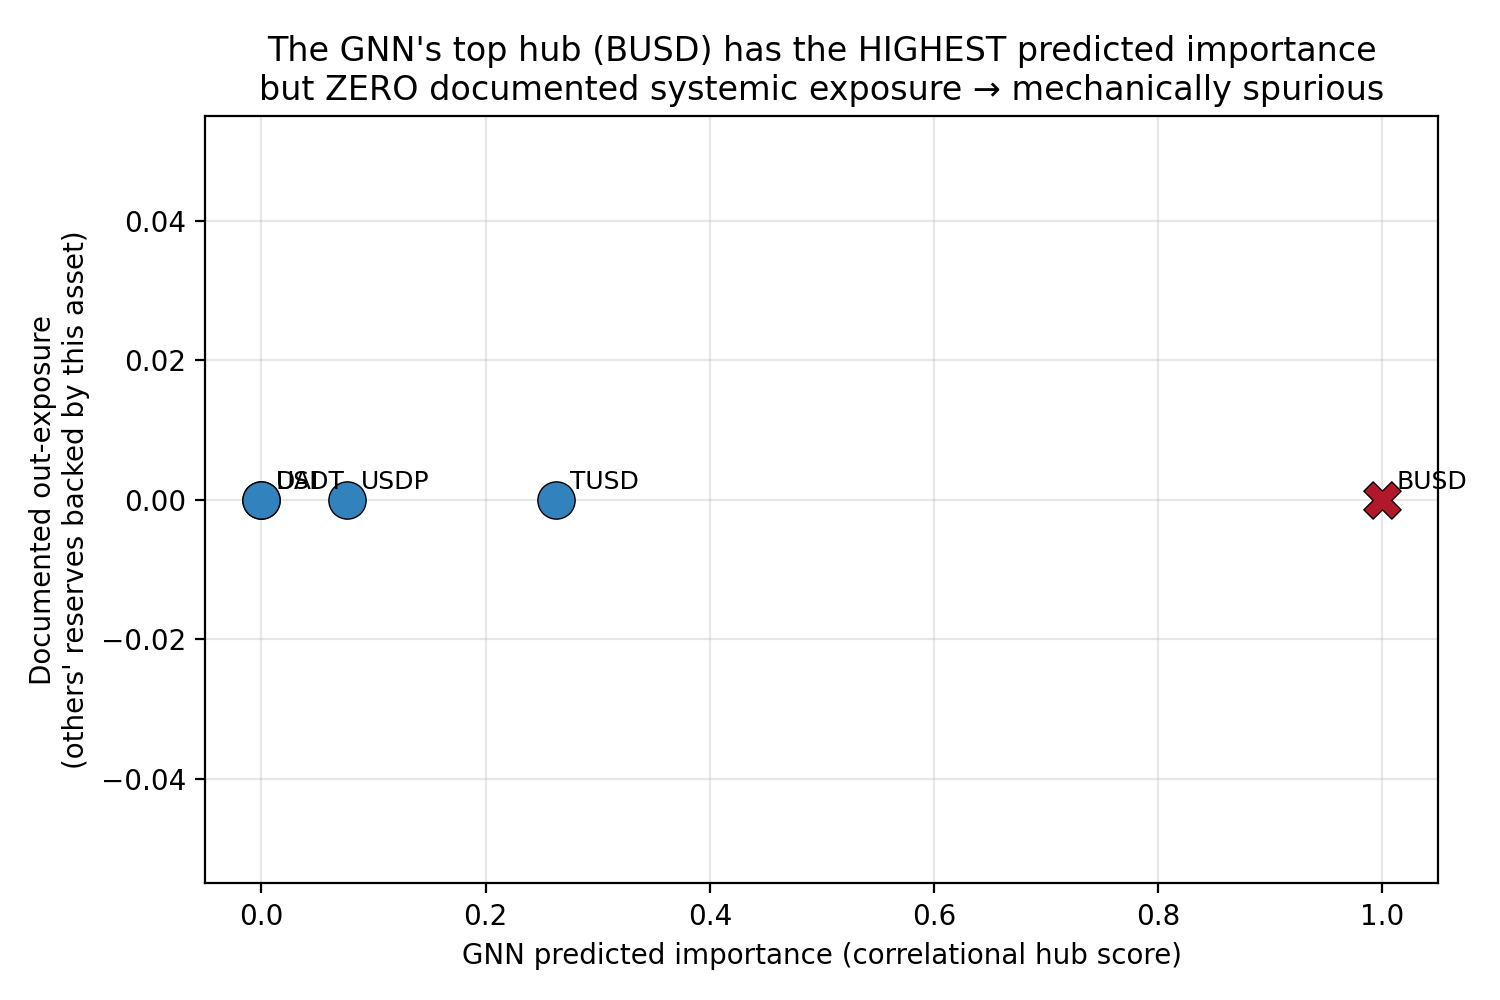
\includegraphics[width=\columnwidth]{figures/02_exposure.png}
\caption{The GNN's top hub (BUSD) has the highest predicted importance but \emph{zero} documented
systemic exposure---no stablecoin's peg depends on it.}
\label{fig:exposure}
\end{figure}

\section{Robustness}
\paragraph{(1) Calibration uncertainty.} Under $\pm30\%$ perturbation of $(c,\kappa,W)$ over 60
draws, USDC is the top causal node $100\%$ of the time and BUSD stays inert $100\%$.
\paragraph{(2) Strategic agents.} We add an endogenous adaptive redeemer (redemptions accelerate
past a threshold, destabilizing) and a capital-capped arbitrageur (a peg-restoring force subject
to limits-to-arbitrage, stabilizing). The redeemer amplifies contagion $7.7\times$ and the
arbitrageur damps it, but across all four agent configurations the origin stays the top causal
node and BUSD stays inert. The \emph{intervention} ranking, however, flips: a circuit breaker
overtakes reserve-strengthening ($95\%$ vs $30\%$) once runs are self-reinforcing, so static-agent
analysis would mis-rank policies (a Lucas-critique check).
\paragraph{(3) Structure derivation.} The estimated and documented networks agree on the marquee
result (\S5).
\paragraph{(4) Placebo control.} On synthetic data with known ground truth
(Fig.~\ref{fig:placebo}), the knockout assigns causal $\Delta=0.139$ to true transmitters and
\emph{exactly zero} to a planted spurious co-mover that correlation centrality cannot distinguish.
The method recovers ground truth, so the real-data refutation is a property of the method, not an
artifact.

\begin{figure}[t]
\centering
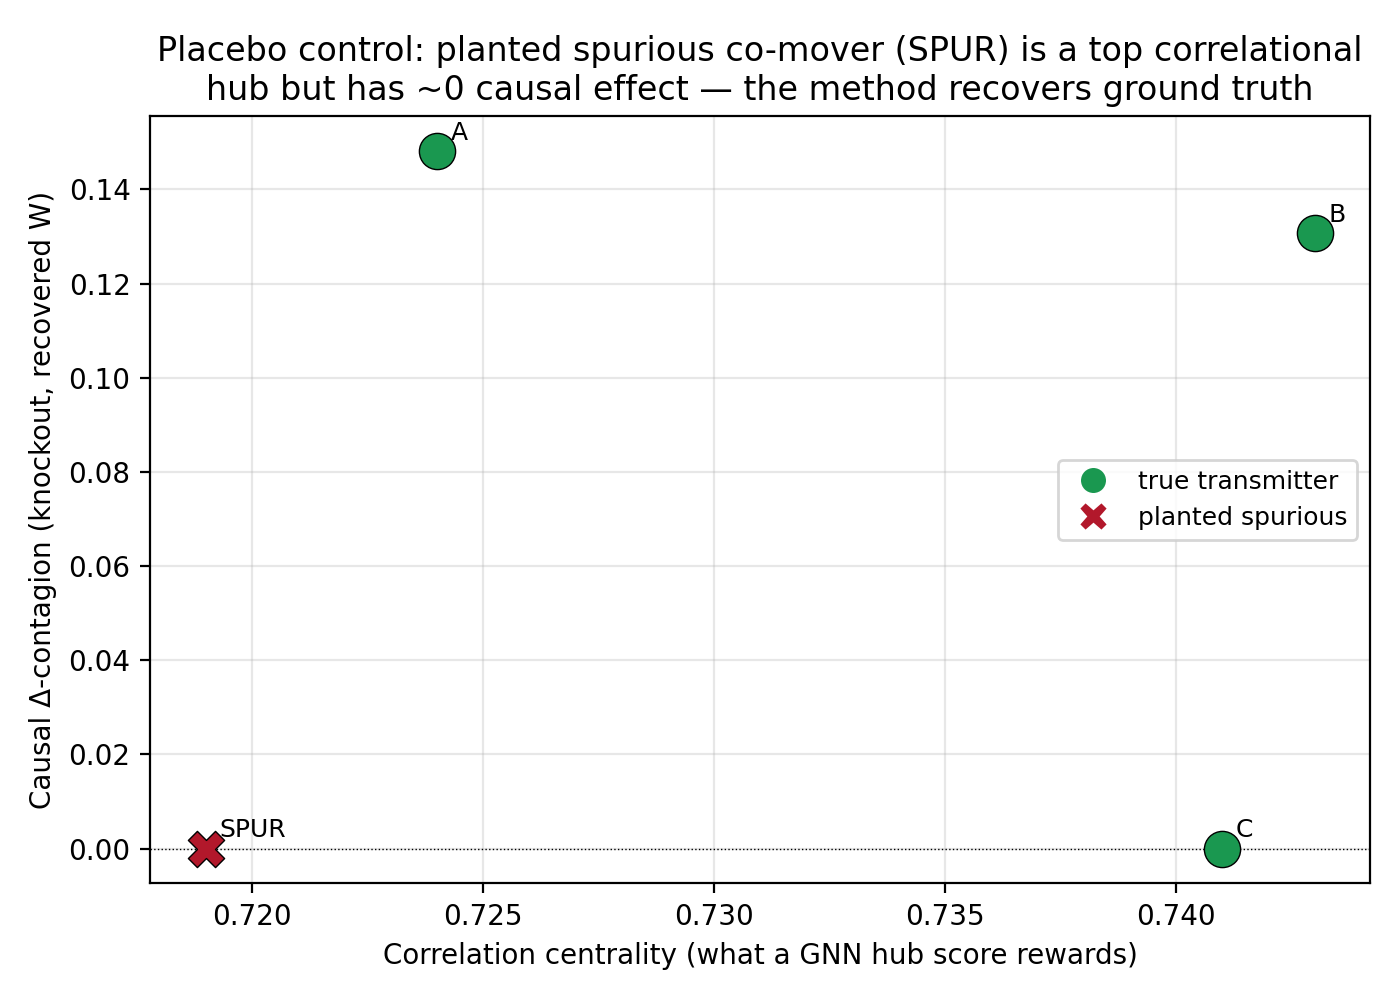
\includegraphics[width=\columnwidth]{figures/03_placebo.png}
\caption{Placebo control. A planted spurious co-mover (SPUR) is correlationally central but
causally inert; the knockout recovers ground truth.}
\label{fig:placebo}
\end{figure}

\begin{figure}[t]
\centering
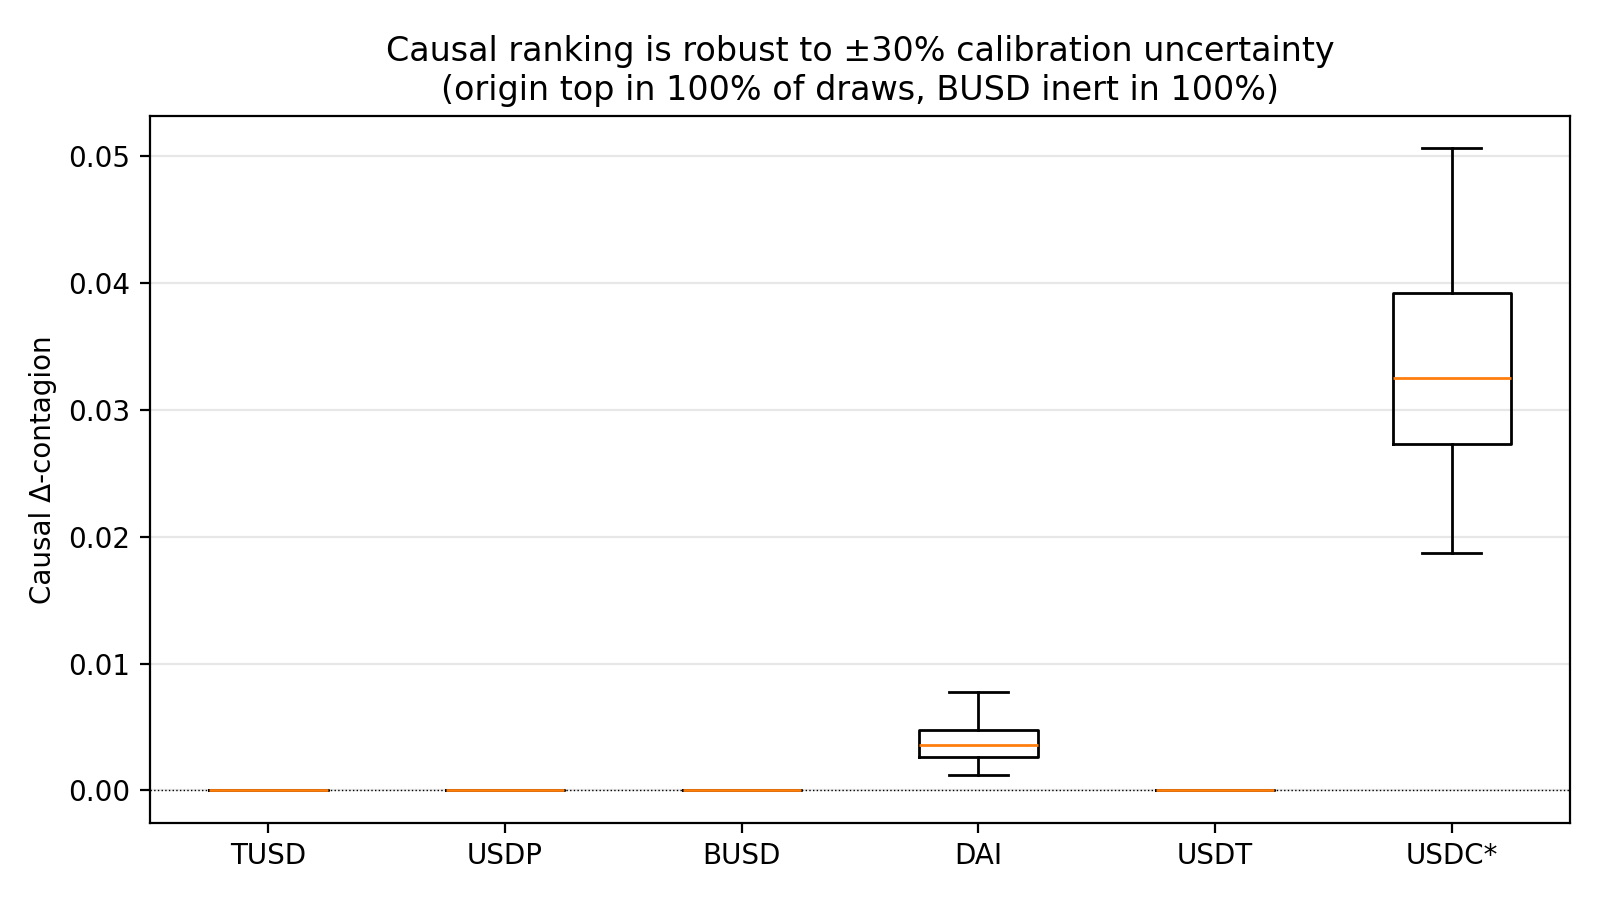
\includegraphics[width=\columnwidth]{figures/05_robustness.png}
\caption{Causal $\Delta$-contagion per node under $\pm30\%$ calibration uncertainty: the origin
dominates and BUSD is pinned at zero across draws.}
\label{fig:robust}
\end{figure}

\paragraph{Generalization.} Across crises (Fig.~\ref{fig:multi}) the GNN's top hub \emph{equals}
the causal driver once (Terra) but \emph{diverges} twice (SVB, USDT-May), so correlational
rankings are unreliable and the causal test is necessary. A static, documented quantity---
out-exposure---ranks causal importance better than the learned GNN score (Spearman $0.20$ vs
$0.09$), and the GNN's top hub is a zero-exposure (structurally non-transmitting) node in $3/5$
episodes.

\begin{figure}[t]
\centering
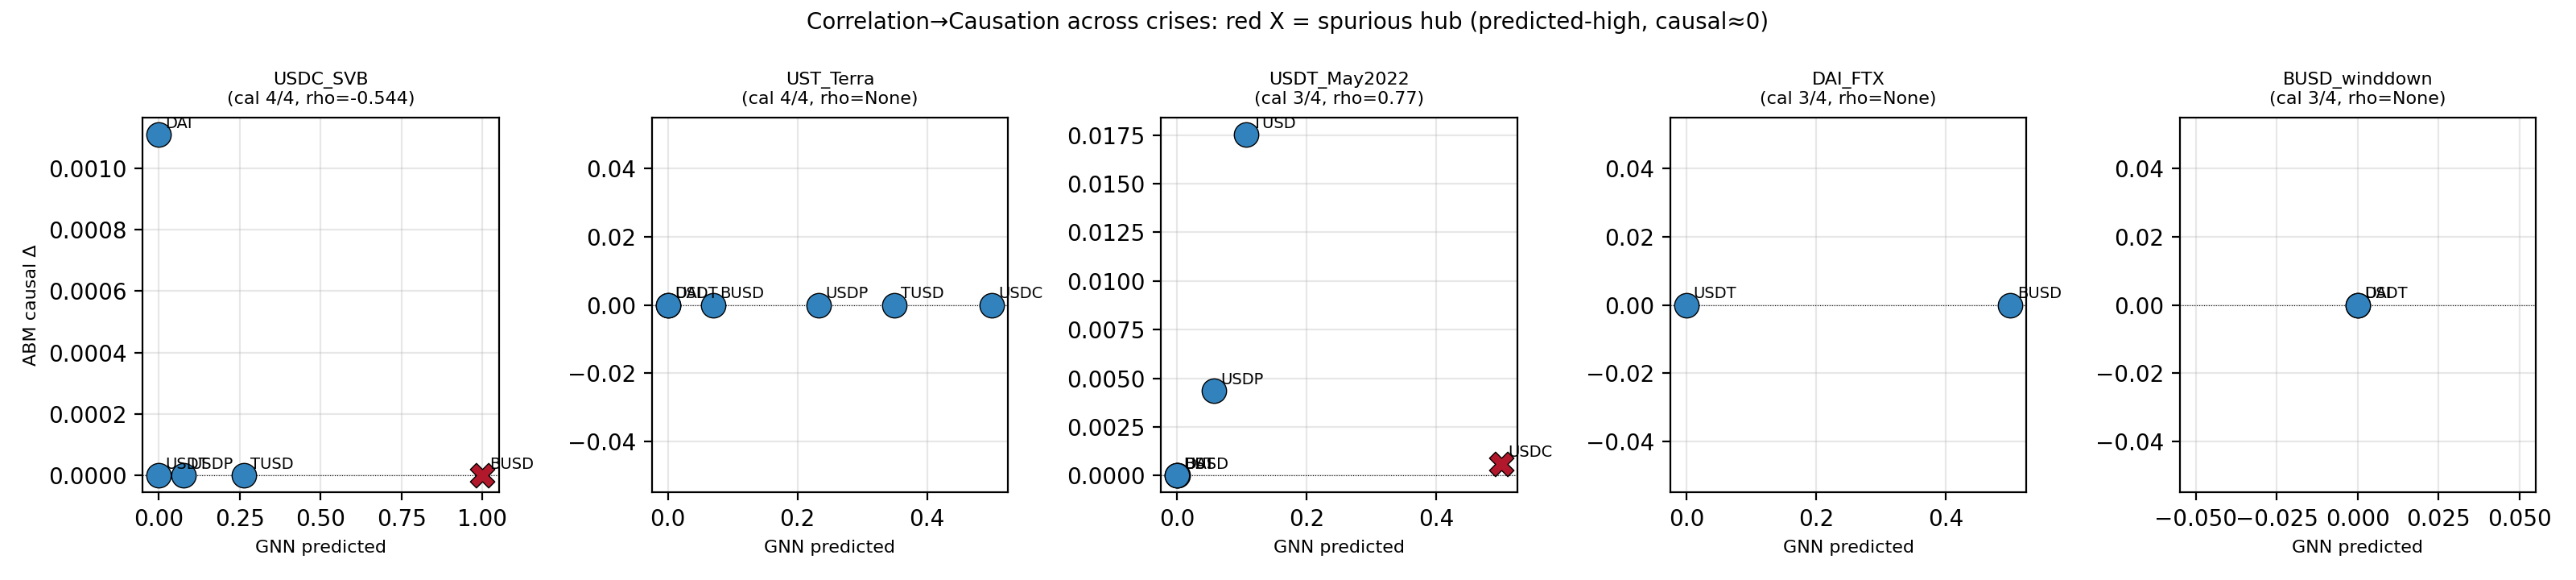
\includegraphics[width=\columnwidth]{figures/06_multi_episode.png}
\caption{The correlation-vs-causation map across crises. Red $\times$ marks a spurious hub
(predicted-high, causal-$\approx 0$).}
\label{fig:multi}
\end{figure}

\section{Policy}
Targeted protection of USDC cuts contagion $100\%$; reserve-strengthening USDC $\times20$ cuts
$89\%$; a circuit breaker $85\%$; redemption gating $100\%$. Protecting or strengthening BUSD cuts
$0\%$ at every intensity. The budget result is stark (Fig.~\ref{fig:interventions}): a regulator
who backstops one venue by the GNN's correlational ranking protects BUSD ($0\%$); by the causal
ranking protects USDC ($100\%$). A PPO regulator given only transmission-network features---no
causal labels---learns to allocate its reserve budget USDC $1.0$ / DAI $0.48$ / \textbf{BUSD
$0.0$}, achieving $93.7\%$ reduction, independently rediscovering the causal targets.

\begin{figure}[t]
\centering
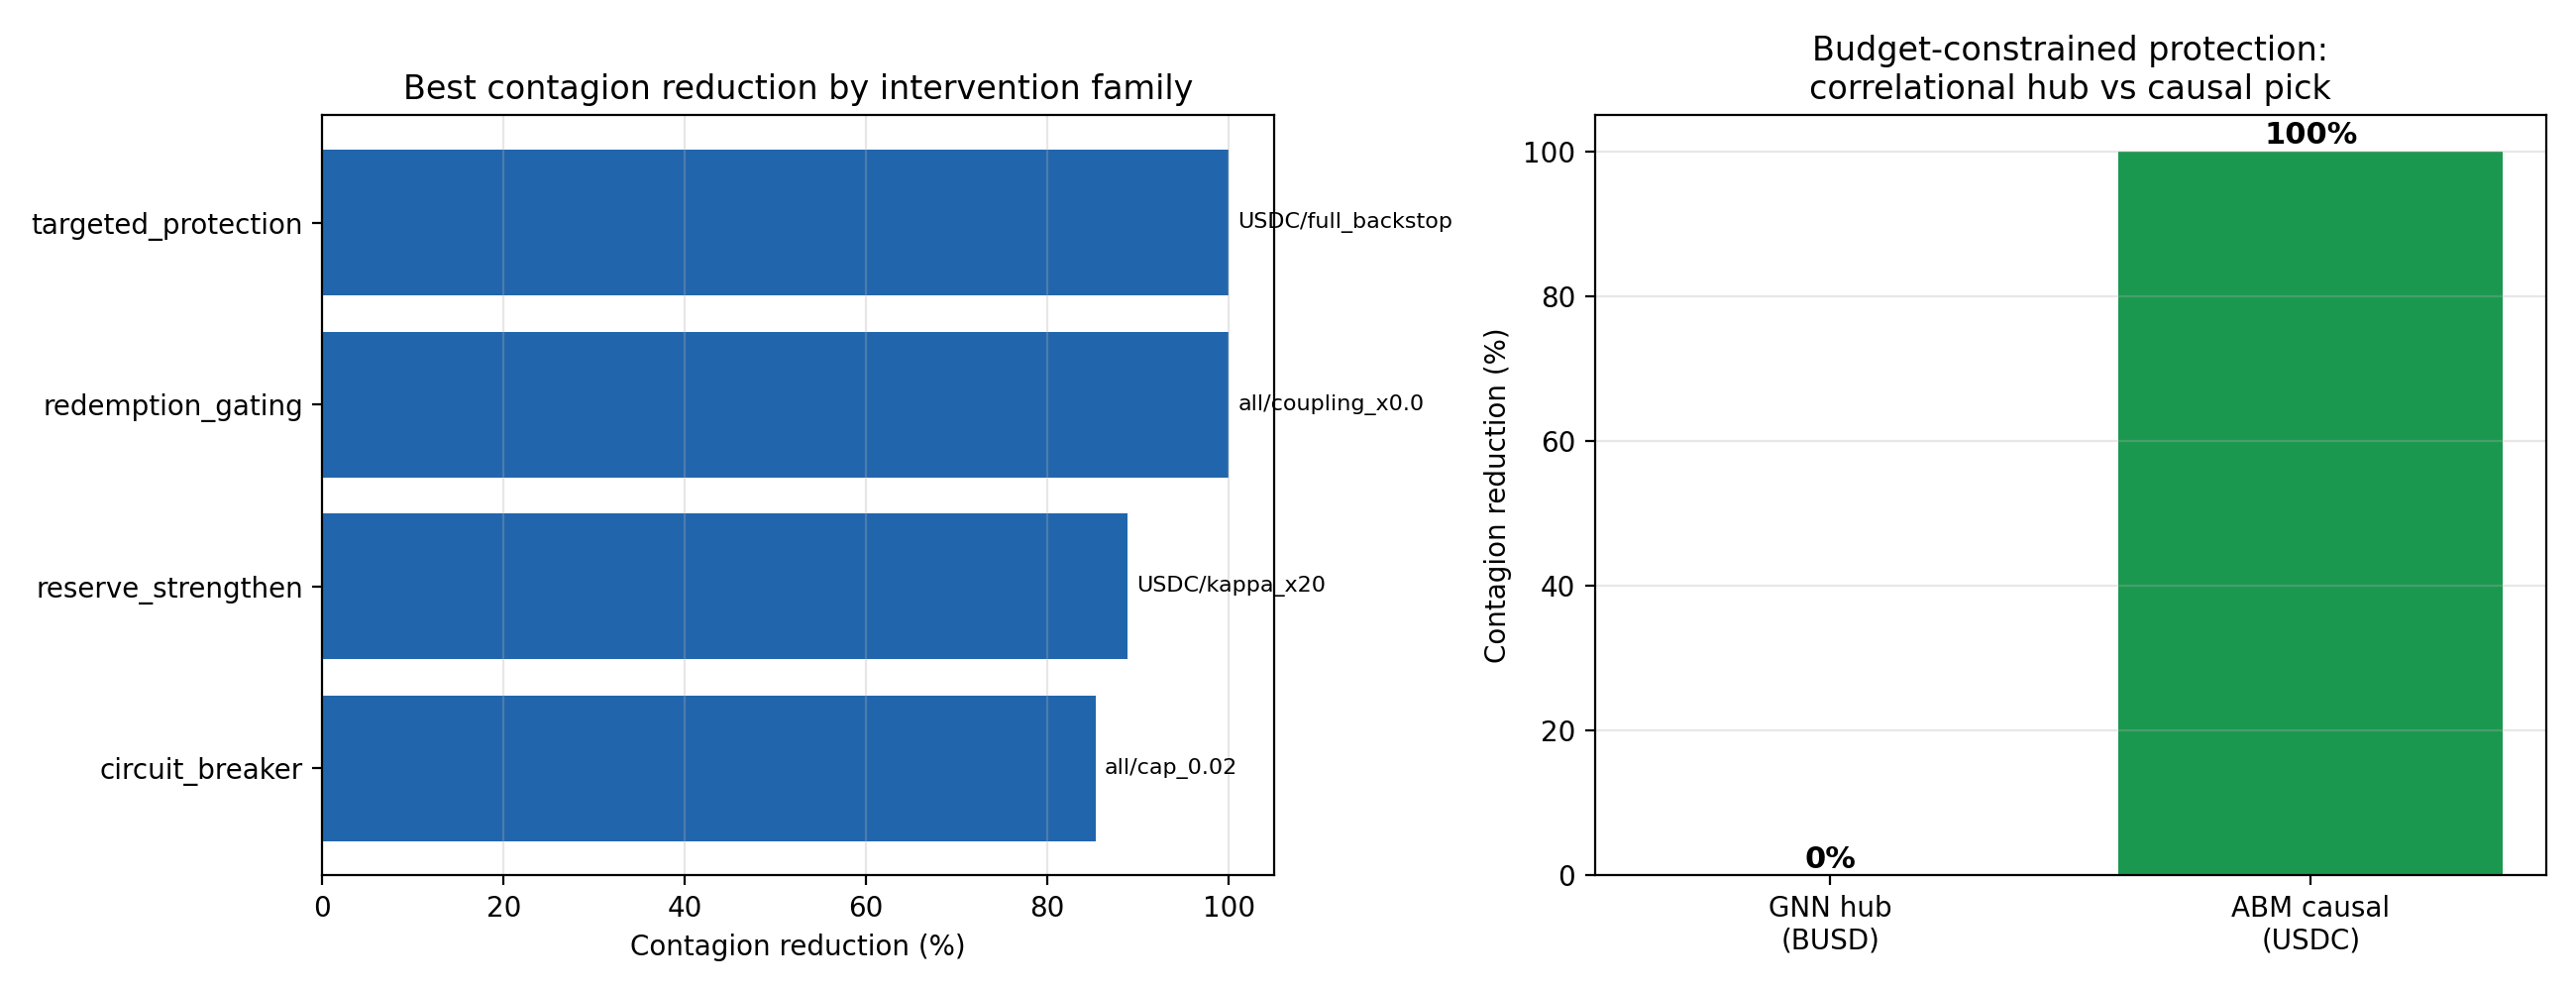
\includegraphics[width=\columnwidth]{figures/04_interventions.png}
\caption{Left: best contagion reduction by intervention family. Right: a one-venue budget spent
on the GNN's correlational hub (BUSD) yields $0\%$; on the causal pick (USDC), $100\%$.}
\label{fig:interventions}
\end{figure}

\section{Limitations}
The model is a reduced form calibrated to a handful of crises; two episodes are too thin to
analyze causally. The estimated $W$ can over-credit thinly traded coins, which is why the
load-bearing claim is the BUSD refutation confirmed independently by the balance sheet. The causal
statements are model-based (structural/interventionist), not from a randomized experiment.

\section{Conclusion}
Contagion hub rankings are correlational, and in the marquee SVB crisis the top-ranked hub causes
\emph{no} contagion because no stablecoin's peg depends on it. A calibrated, balance-sheet-grounded
contagion model supplies the missing causal test, and the disagreement is decisive for policy:
acting on the correlational hub wastes the entire budget the causal target would have spent to
contain the cascade. Contagion analytics intended for intervention should report \emph{validated
causation}, not centrality alone.

\paragraph{Reproducibility.} Every number is produced by committed scripts; \texttt{reproduce.sh}
regenerates all results and figures end-to-end.

\bibliographystyle{ACM-Reference-Format}
\bibliography{references}

\end{document}
